\Exhibit{GdeHome}{
    Главная страница Google Developer Experts
}

Это скриншот главной страницы сообщества Google Developer Experts.

Вверху написано \Quote{Присоединитесь к глобальному сообществу из более чем 1,000 профессионалов}.
Это даёт грубую оценку количества экспертов в мире
и показывает редкость статуса `Google Developer Expert'.

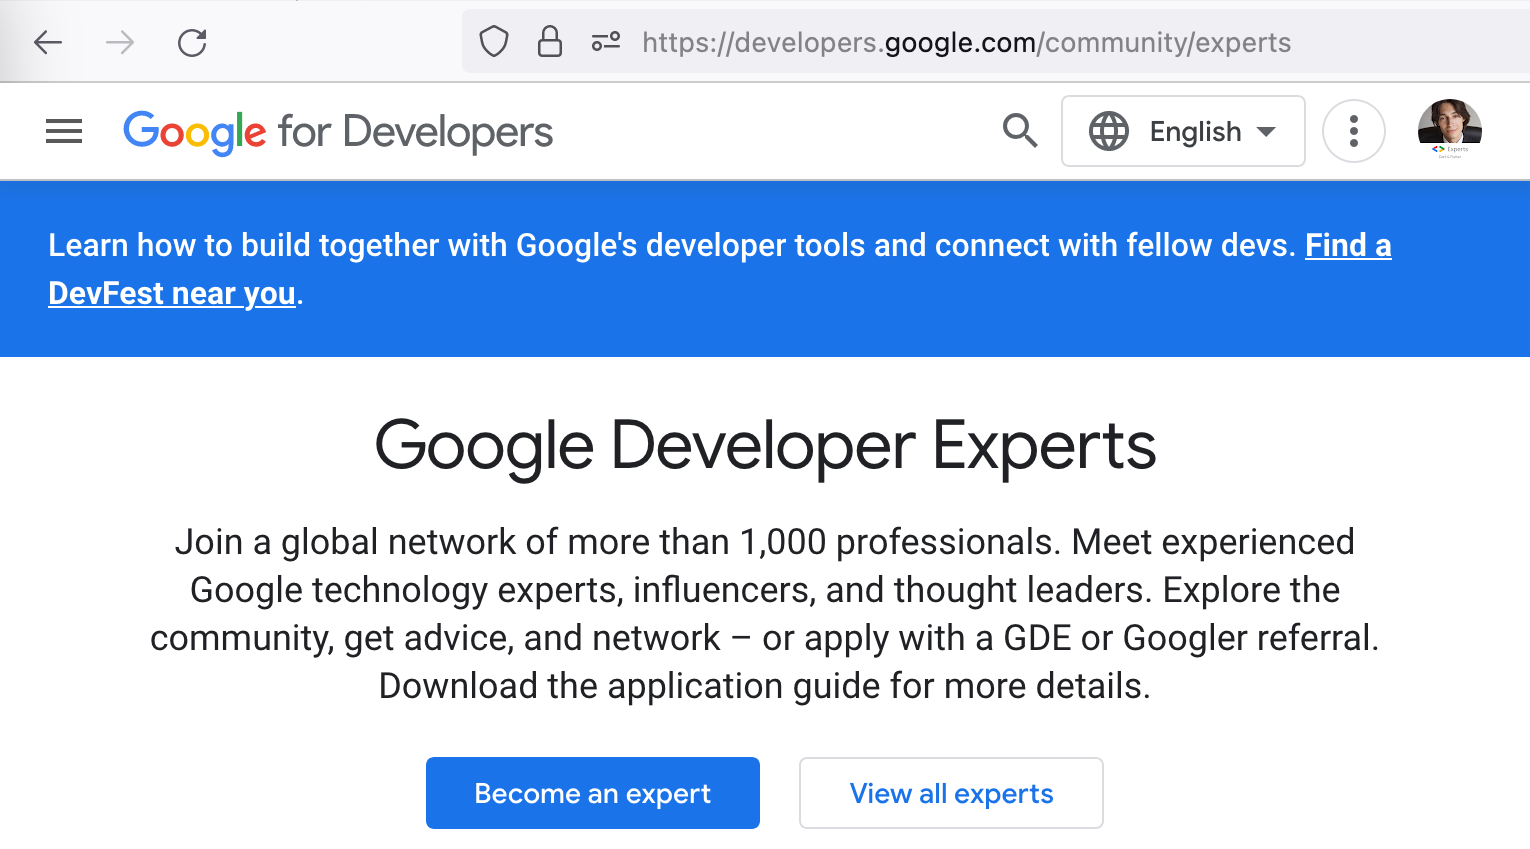
\includegraphics[width=\textwidth]{home-p1}
\WillContinue

\pagebreak

Внизу страницы -- раскрываемая секция \Quote{Кто может стать Google Developer Experts?}

\Continuing

\includegraphics[width=\textwidth]{home-bottom}

В ней среди требований два ключевых:

\ParagraphQuote{%
    Твёрдый опыт в области, для которой существует технология Google, например: Android,
    Google Cloud, Machine Learning, Web и другие.%
}
\ParagraphQuote{%
    Показать значительный вклад в сообщество разработчиков, включая,
    но не ограничиваясь выступлениями на мероприятиях, публикацией контента,
    менторством других разработчиков и компаний.%
}

Это доказывает, что для одобрения необходимы высокие достижения.

Внизу страницы -- раскрываемая секция \Quote{Как подать заявку?}.
В ней ссылка `discuss your eligibility', которая ведёт на подробное описание процесса.
Оно показано далее в \ExhibitRef{GdeApplicationGuide}.

\pagebreak
